%%%%%%%%%%%%%%%%%%%%%%%%%%%%%%%%%%%%%%%%%%%%%%%%%%%%%%%%%%%%%%%%%%%%%%%%%%%%%%%%
% Template for USENIX papers.
%
% History:
%
% - TEMPLATE for Usenix papers, specifically to meet requirements of
%   USENIX '05. originally a template for producing IEEE-format
%   articles using LaTeX. written by Matthew Ward, CS Department,
%   Worcester Polytechnic Institute. adapted by David Beazley for his
%   excellent SWIG paper in Proceedings, Tcl 96. turned into a
%   smartass generic template by De Clarke, with thanks to both the
%   above pioneers. Use at your own risk. Complaints to /dev/null.
%   Make it two column with no page numbering, default is 10 point.
%
% - Munged by Fred Douglis <douglis@research.att.com> 10/97 to
%   separate the .sty file from the LaTeX source template, so that
%   people can more easily include the .sty file into an existing
%   document. Also changed to more closely follow the style guidelines
%   as represented by the Word sample file.
%
% - Note that since 2010, USENIX does not require endnotes. If you
%   want foot of page notes, don't include the endnotes package in the
%   usepackage command, below.
% - This version uses the latex2e styles, not the very ancient 2.09
%   stuff.
%
% - Updated July 2018: Text block size changed from 6.5" to 7"
%
% - Updated Dec 2018 for ATC'19:
%
%   * Revised text to pass HotCRP's auto-formatting check, with
%     hotcrp.settings.submission_form.body_font_size=10pt, and
%     hotcrp.settings.submission_form.line_height=12pt
%
%   * Switched from \endnote-s to \footnote-s to match Usenix's policy.
%
%   * \section* => \begin{abstract} ... \end{abstract}
%
%   * Make template self-contained in terms of bibtex entires, to allow
%     this file to be compiled. (And changing refs style to 'plain'.)
%
%   * Make template self-contained in terms of figures, to
%     allow this file to be compiled. 
%
%   * Added packages for hyperref, embedding fonts, and improving
%     appearance.
%   
%   * Removed outdated text.
%
%%%%%%%%%%%%%%%%%%%%%%%%%%%%%%%%%%%%%%%%%%%%%%%%%%%%%%%%%%%%%%%%%%%%%%%%%%%%%%%%

\documentclass[letterpaper,twocolumn,10pt]{article}
\usepackage{usenix2019_v3}

% to be able to draw some self-contained figs
\usepackage{tikz}
\usepackage{amsmath}
\usepackage{comment}
\usepackage{pdfcomment}
\usepackage{color}
\usepackage{graphicx}
\usepackage{caption}
\usepackage{subcaption}
\usepackage{threeparttable}
\usepackage{multirow}
\usepackage{booktabs}
\usepackage{verbatim}
\usepackage{epstopdf}
\usepackage{rotating}
\usepackage{listings}
\usepackage{listing}
\usepackage{paralist}
\usepackage{arydshln}
\let\labelindent\relax
\usepackage{enumitem,amssymb}
\usepackage{algpseudocode}% http://ctan.org/pkg/algorithmicx
\usepackage{balance}
\usepackage{endnotes}
\usepackage{xspace}
\usepackage{times}
\usepackage{amsfonts}
\usepackage{pifont}
\usepackage{wasysym}
\usepackage{tikz}
\usepackage{hyperref}
\usepackage{minted}
\usepackage{xcolor}
\usepackage{colortbl}
\usepackage{soul}
\usepackage[normalem]{ulem}
\usepackage{algpseudocode}
\usepackage{algorithm}
\usepackage{cleveref}
% \usepackage[noadjust]{cite}
% \renewcommand{\citepunct}{,\penalty\citepunctpenalty\,}
% \renewcommand{\citedash}{--}

\newcommand{\spartacus}{{Spartacus}\xspace}

% inlined bib file
% \usepackage{filecontents}

% %-------------------------------------------------------------------------------
% \begin{filecontents}{\jobname.bib}
% %-------------------------------------------------------------------------------

% \end{filecontents}

%-------------------------------------------------------------------------------
\begin{document}
%-------------------------------------------------------------------------------

%don't want date printed
\date{}

% make title bold and 14 pt font (Latex default is non-bold, 16 pt)
\title{Spartacus: Cloak Users Against Cloaked Phishing Websites}

%for single author (just remove % characters)
% \author{
% {\rm Your N.\ Here}\\
% Your Institution
% \and
% {\rm Second Name}\\
% Second Institution
% % copy the following lines to add more authors
% % \and
% % {\rm Name}\\
% %Name Institution
% } % end author

\maketitle

%-------------------------------------------------------------------------------
\begin{abstract}
%-------------------------------------------------------------------------------
% Your abstract text goes here. Just a few facts. Whet our appetites.
% Not more than 200 words, if possible, and preferably closer to 150.
Phishing has been the top online attack nowadays.
Phishers implement cloaking techniques to evade detection from anti-phishing systems by checking profiles from HTTP requests in server side as well as from browsers in client side.
The anti-phishing ecosystem has been devoting to reveal real phishing content behind cloaks.
However, it has few progress because phishers can always enrich their fingerprinting database by adding new rules to distinguish traffics from the ecosystem and hence evade the visit.

According to the situation where cloaking techniques are widely implemented in phishing attacks and the goal of anti-phishing is to prevent Internet users to see phishing contents, we consider the security problem from a different perspective: instead of trying best to reveal phishing content, we can leverage the cloaking techniques in phishing to prevent users to see phishing content. In this work, we propose \emph{Spartacus}, a framework that disguise Internet users as anti-phishing crawlers to request web page content of a suspicious URL, while remain users' own profiles on visiting whitelisted websites.

\textcolor{blue}{Evaluation plan:}
We evaluated Spartacus from different aspects: (1) Effectiveness: we have two groups open reported phishing websites, one with normal browser, the other with ``Spartacused'' browser, for three months. We expect to show Group 1 saw way more phishing than Group 2.
(2) Efficiency: Two groups visit same amount of websites to test the latency of Spartacus.
Also we use Spartacus to visit legitimate websites to evaluate the impact (layout of the websites).
Then, we evaluate how difficult is to maintain our Spartacus system.
(3) adversarial mindset
(4) other fingerprints to get

\end{abstract}

\section{Introduction}

The security community has made efforts researching on phishing attacks,
but attackers still make profits using phishing websites and continuously harm the victims they target and the organizations they mimic~\cite{ho2019detecting, van2019cognitive}.
According to Google Transparency report, phishing attacks have replaced online malware to be the most prevalent web-based threat~\cite{googletransparencyreport, solutions2019verizon}.
Nowadays, phishing websites continue to grow in sophistication and hence can bypass modern defensive methodologies.
Therefore, the current anti-phishing ecosystem leaves advanced phishing websites ``golden hours'' to damage the whole Internet community~\cite{oest2020sunrise}.

Phishing websites adopt \emph{evasion} techniques to delay or evade detection by automated anti-phishing systems in the cat-and-mouse game,
which contribute to maximize phishers' return-on-investment~\cite{thomas2017data}.
The evasion techniques, also known as~\emph{cloaking}, 
% implemented in phishing websites, 
attempt to distinguish the visits from potential victims out of those from anti-phishing crawlers.
The cloaking techniques include two categories: server-side~\cite{oest2018inside} and client-side~\cite{zhang2021crawlphish}.
Server-side cloaking techniques reside in phishing servers and perform based on the HTTP request. 
Among them, many phishing kits implement fingerprinting cloaking, to identify visits through the items in the request, such as IP, User-Agent, and Referrer~\cite{oest2018inside}.
The client-side ones take into effect based on the execution of JavaScript in user's browser.
The cloaking techniques show real phishing content to visitors who they decide as ``real human,'' while display a benign-looking web page to those who are identified as ``anti-phishing crawler.''
The damage brought by these phishing websites' efforts is not only that they steal just account numbers and passwords,
but that the phishing websites nowadays try to dump all information including victim's identity~\cite{thomas2017data}.
Thus, the cloaked phishing websites cause a wider damage to the whole society and are very difficult to effectively and efficiently mitigate~\cite{oest2020sunrise, zhang2021crawlphish}.

According to Oest et al.~\cite{oest2020sunrise}, such sophisticated phishing websites cause majority of real-world harm.
Thwarting phishers' evasion efforts is, thus, treated by the anti-phishing ecosystem as a very important issue.
Currently, they think that correct web page retrieval and timely detection is the key to successful mitigation~\cite{oest2020sunrise, zhang2021crawlphish}.
Following this trajectory, prior research has proposed methodologies categorizing and mitigating cloaking techniques in phishing~\cite{oest2018inside, oest2019phishfarm, zhang2021crawlphish}.
However, the server-side cloaking techniques can still defeat key ecosystem defenses such as blacklist-based mechanism~\cite{oest2019phishfarm}.
With so many filtering conditions in the cloaking techniques,
it is very difficult for the content-based anti-phishing systems to acquire real phishing content in a large scale~\cite{oest2018inside, oest2020phishtime},
because anti-phishing systems need to enumerate countless HTTP profiles to visit the phishing websites, in order not to bypass the cloaking techniques.
In this way, phishers can still be beneficial from the cloaking techniques.
% This magnifies an issue that current anti-phishing systems cannot provide a reliable protection for users against phishing websites with cloaking techniques.


We first perform an automated evaluation, to analyze the prevalence of fingerprinting cloaking techniques in phishing kits.
% and the ability of current anti-phishing systems against phishing websites.  
In total, we analyzed 2,933 phishing kits from \emph{phishunt.io}~\cite{phishunt} and Cisco, and discovered that 96.52\% (2,831) of them contain fingerprinting cloaking techniques, which shows that such evasion is very prevalent within our dataset.
So, since we know to expect fingerprinting cloaking in phishing, how about we consider the problem from a different angle:
the ultimate goal to mitigate or defeat phishing is to prevent potential victims from seeing any phishing content.
So why do we devote ourselves trying to sneak through all the challenges that cloaking techniques set and reach to the phishing content?
Why not trigger the cloaking techniques from the client-side and let phishing websites return a benign-looking web page to users?
In this way, users will not see phishing content in real time, and a lose-lose situation is shown to phishers because they cannot differentiate visits from between users and anti-phishing crawlers.

To this end, we propose \spartacus, a framework that disguises Internet users as anti-phishing crawlers from the client-side to request web page content of a suspicious URL, while remain users' own profiles on visiting benign websites.
% Before visiting a URL, \spartacus queries the domain information, such as reputation, to decide whether to mutate the HTTP profile.
% If not, 
\spartacus allows the request sent with user's default profile when visiting trustworthy websites.
When visiting suspicious websites, \spartacus mutates the items in the HTTP profile such as User-Agent string, Referrer, or IP (through a proxy server) to make it look like an anti-phishing crawler.
% that will be inspected by cloaking techniques in the phishing server before sending requests to suspicious URLs.
When the fingerprinting cloaking script examines the HTTP request, it will identify that the visit is from an anti-phishing infrastructure, and will return a benign-looking web page to users.
% \spartacus traps phishers into a dilemma: phishers can choose to use more precise conditions to identify traffic, for example, they mark a visitor as crawler only when IP \texttt{AND} User-Agent are match.
% This will allow more traffic in and bypass \spartacus to some extent,
% but such option will make anti-phishing crawlers easy to sneak through the cloaking techniques.
% 


Then, we deploy the \spartacus framework in large-scale to evaluate the effectiveness, efficiency, and potential impact on users' browsing activity.
In total, over a period of nine months from late-2020 to mid-2021, \spartacus visits \totalphishing phishing websites in the wild and evades 82.28\% of them.
In addition, the \spartacus framework as a browser extension has negligible reaction and scripting time, compared with other popular plugins~\cite{exthouse}, and hence it does not slow down the web page rendering of the benign websites.
People who use \spartacus will not perceive its existence.
At last, we analyze the performance of \spartacus on benign websites both automatically and manually.
We found that with \spartacus installed, the benign website can still display properly.
Functionalities in the website such as buttons/links, online chat, register/login, shopping cart and checkout can correctly perform without any error.

We also evaluate the support from current anti-phishing systems against phishing websites.
We totally submit 45,526 phishing websites to anti-phishing systems when \spartacus visits them and query the result every 15 minutes.
Among the submitted phishing websites, 24,154 can be evaded by \spartacus but cannot detected by anti-phishing systems;
16,698 can be evaded and detected;
4,598 cannot be evaded but can be detected;
and 76 can neither be evaded nor detected.
% to test if they can timely detect the phishing websites \spartacus cannot evade.
Comfortingly, we notice that current anti-phishing systems can timely (0.36 hours) detect and blacklist 98.33\% of phishing websites that show phishing content to any HTTP profile (basic phishing).
However, when encountering with advanced phishing websites with fingerprinting cloaking (showing different content to different profile), they do not perform well.
Only 40.87\% of the websites can be detected, and the detection time (2.58 hours) is more than eight times as that on basic phishing.

The proposal of \spartacus traps phishers into a dilemma:
to bypass \spartacus, phishers can only disable some criteria and allow more traffic in, because they fail to tell the difference between victim traffic and crawler traffic.
However, this loose strategy will enable more crawlers in and hence the websites can be blocked faster.
On the other hand, they can choose to build up more criteria, which allows less traffic, but it is easy for \spartacus to trigger.
Our \spartacus framework can be further embedded in web browsers to continuously protect users from fingerprinting-cloaked phishing websites.
The methodology can not only directly reduce the ``golden hour'' current anti-phishing systems leave for phishers,
but also trap the attackers into a dilemma that they have to think of another approach to mitigate.
Our contributions are thus as follows:

\begin{itemize}
    \item An analysis of modern phishing kits to understand the prevalence of fingerprinting cloaking techniques.
    \item An automated framework that can evade phishing websites with fingerprinting cloaking while negligibly impact user's browsing activity.
    \item An evaluation for \spartacus as a browser extension to measure its effectiveness and efficiency and that of current anti-phishing systems to reveal the less capability against phishing websites with such evasion.
    % \item A dilemma where phishers cannot differentiate crawler and human visits and hence lose the chance to lure credentials.
\end{itemize}

\section{Background}
\label{s:background}

\cloakingTypes



Over past several decades, the anti-phishing ecosystem has proposed and leveraged a number of techniques to detect and migitate phishing attacks~\cite{oest2018inside}.
Techniques such as URL~\cite{bin2010dns, blum2010lexical, huang2012svm, khonji2011novel} and web page content analysis~\cite{wu2006web, zhang2007cantina, zhang2011textual, bilge2011exposure, canali2013role} have raised the defensive level of the ecosystem and productized implementations such as URL blacklists, malicious infrastructure analysis, and e-mail spam filter.

Commodity URL blacklists such as Google Safe Browsing~\cite{whittaker2010large} and Microsoft SmartScreen~\cite{smartscreen} reinforces the backend of the anti-phishing ecosystem, which warn users with prominent sign indicating that the websites ahead are suspicious when phishing URL is detected and blacklisted.
Evasion techniques, also known as cloaking techniques, are widely leveraged in phishing attacks to delay or disable detection by anti-phishing systems~\cite{liang2016cracking, oest2019phishfarm, oest20phishtime}.

% \subsection{Server-side Cloaking in Phishing}


Attackers often implement \emph{cloaking techniques} to evade detection by the anti-phishing ecosystem.
Typically, phishing websites with evasion display benign web page content if they suspect the visit originates from a security infrastructure~\cite{wu2005cloaking}.
There are two categories of cloaking techniques, namely server-side and client-side (\autoref{tab:cloakingtypes} shows categories of each type).
Client-side evasion techniques distinguish visitors to display different web page content by executing JavaScript snippets in user's browser~\cite{zhang2021crawlphish}.
Server-side cloaking techniques, on the other hand, identify visits from anti-phishing systems through information in HTTP requests~\cite{oest2018inside, invernizzi2016cloak}.
Typically, server-side cloaking is also known as fingerprinting cloaking, including network, browser, and context~\cite{invernizzi2016cloak}.
\autoref{fig:fp_cloaking} shows how fingerprinting cloaking techniques are used in phishing websites.
Cloaking code embedded in the phishing server fingerprints the profile in the HTTP request and responds different web page content based on the identification of visitors (as either potential victims or anti-phishing crawlers).

Researchers detect and categorize client-side cloaking techniques in phishing by force-executing the payload JavaScript snippets~\cite{zhang2021crawlphish}.
To bypass server-side cloaking techniques in phishing attacks, the anti-phishing systems camouflage themselves as if they are regular visitors.
Only when anti-phishing systems retrieve phishing content, can they classify phishing websites~\cite{xiang2011cantina+,whittaker2010large,smartscreen}.

However, as the development of phishing kits, the size of blocklist in the phishing kit increases.
As shown in~\autoref{fig:servercloaking}, any match of the IP addresses or hostnames in the blocklist will result in an error web page, such as 404 Page Not Found.
Hence, anti-phishing systems can trigger fingerprinting cloaking techniques in the phishing server easily.
As a result, they cannot properly retrieve phishing web page content, which leads to a mis-classification.
Moreover, according to the analysis from Oest et al.~\cite{oest2020sunrise}, it takes anti-phishing crawlers an average of six hours to mark a phishing website as malicious.
The duration is even longer till the last victim visit (18 hours).
Such long reaction time has left phishers a golden hour to hurt Internet users.

We can consider the problem from a different angle: phishers try their best to evade visits from anti-phishing ecosystem, so how about Internet users camouflage themselves as crawlers when visiting phishing websites?
In this way, users can only see an error web page and never submit credentials to phishers.
It also shrinks the reaction time to blacklist them.


% \subsection{Mitigations Against Advanced Phishing}

% \subsection{Limitations of Mitigations}

\begin{figure}
\centering
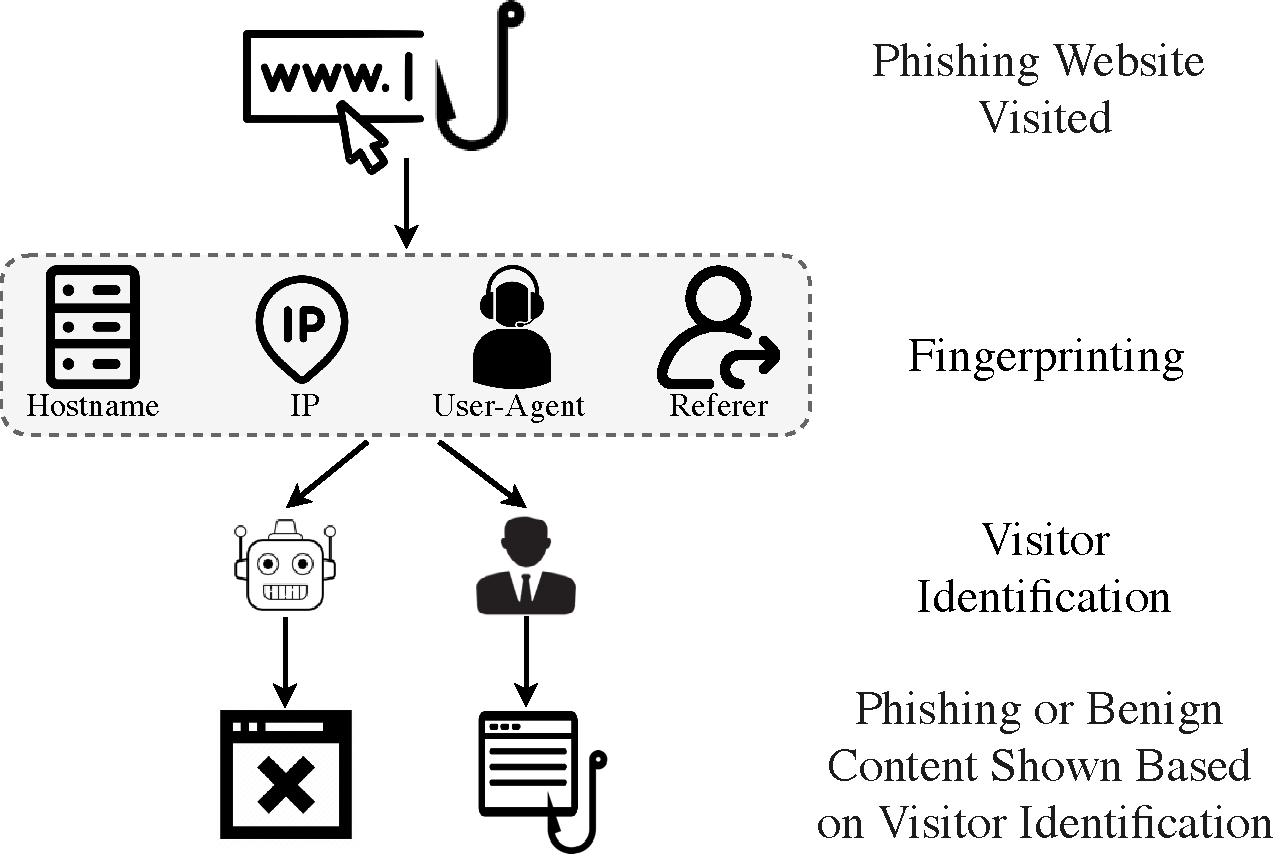
\includegraphics[width=.9\linewidth]{figs/fp_cloaking.pdf}
\caption{Typical operation of fingerprinting cloaking in phishing websites.}
\label{fig:fp_cloaking}
% \vspace{-15pt}
\end{figure}
\section{Design}

We aim to evade advanced phishing websites from the user end in real time when users visit them.
To this end, we design, implement, and evaluate~\spartacus, a framework that automatically evade malicious websites that implement fingerprint cloaking.

\begin{figure*}
\centering
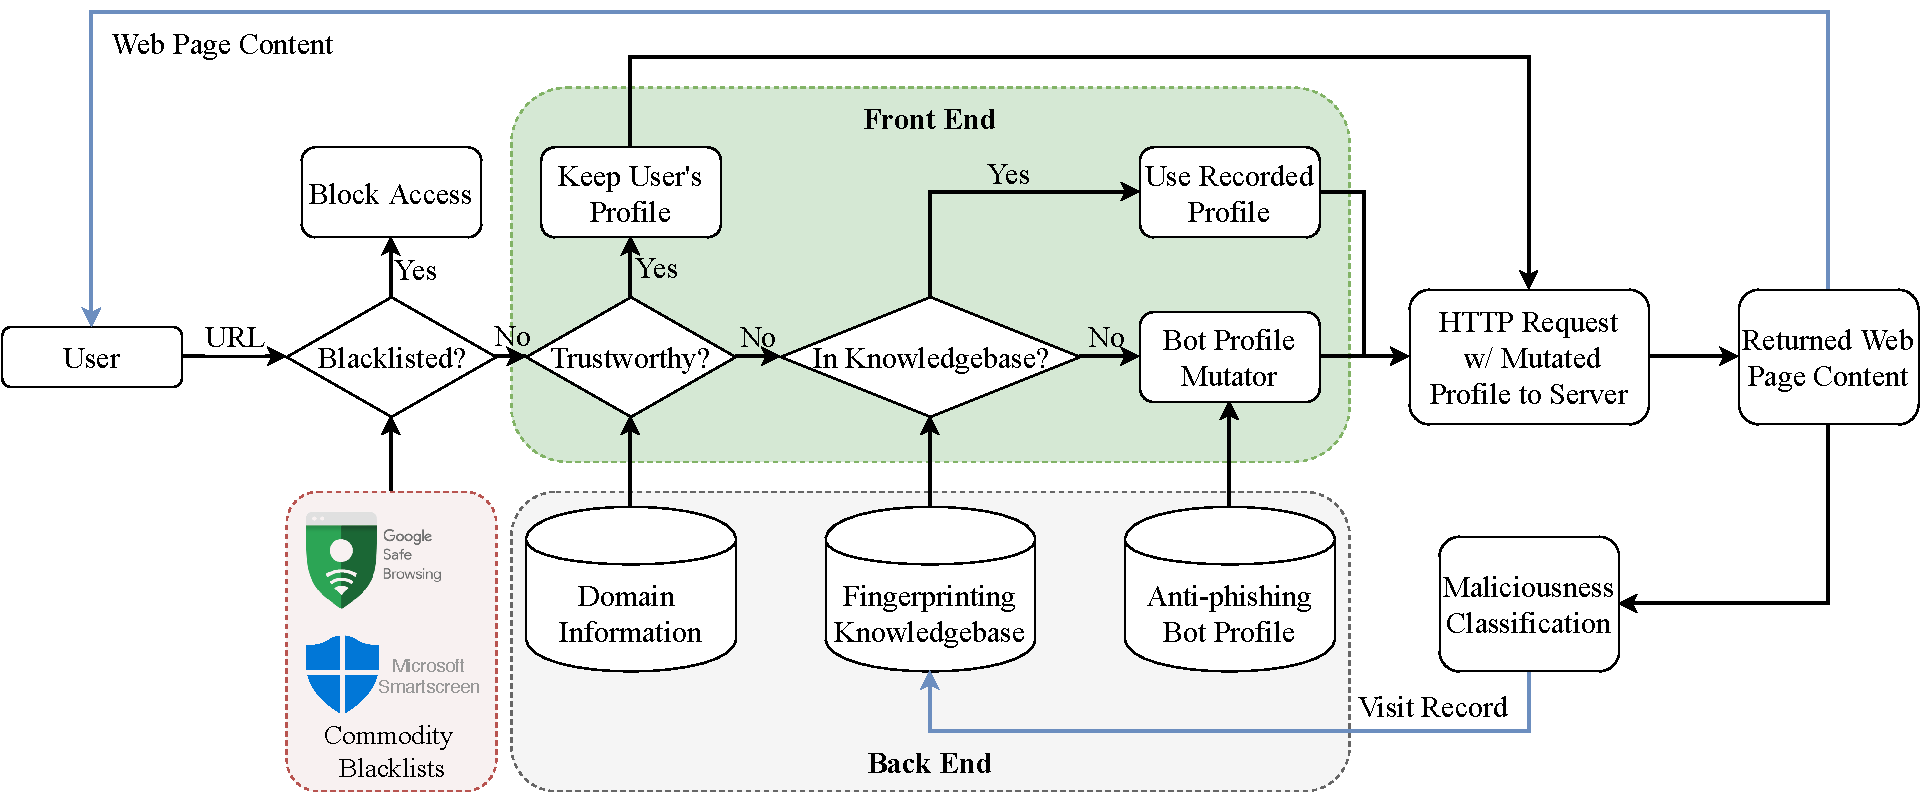
\includegraphics[width=\linewidth]{figs/arch.pdf}
\caption{\spartacus architecture.}
\label{fig:sp_arch}
% \vspace{-10pt}
\end{figure*}

\subsection{Overview}
\autoref{fig:sp_arch} demonstrates the architecture of the \spartacus system.
The whole system consists of two parts, \emph{front end} and \emph{back end}. 
The front end is responsible for filtering whitelisted or blacklisted URLs and mutating profiles in the HTTP request such as user agent. 
In the back end, we maintain several databases to provide support to the front end, including black and whitelist database, which is used to process known URLs, fingerprinting knowledge base, which stores the successful mutation, the anti-phishing bot profile database, which contains the profiles of anti-phishing systems such as google bot, phishing attributes, which is used to distinguish the maliciousness of returned web page content. 

When a user tries to visit a URL, first the URL goes to black and whitelist. 
If the existing record is found, the browser will either block the access or keep user's original profile when requesting the server. 
Otherwise, the front end will query the fingerprinting knowledgebase to see if we have processed the same url before, if found, we will use recorded profile to request the website, if not, we will mutate profile to a bot one. Then with the “spartacus” profile, HTTP request is sent to the server. After getting the page content, we determine whether there is maliciousness. If yes, the browser will show a warning sign to the user, or the web page content will be shown to the user. The knowledge base will be updated accordingly under both situations. 

\subsection{Collection and Maintenance of Back End Databases}

\noindent
\textbf{Black- and whitelist database.}
Blacklist based anti-phishing systems such as Google Safe Browsing and Microsoft SmartScreen have been examining and collecting phishing URLs to warn users before they visit the websites.
We collect known phishing URLs from common blacklists so that \spartacus can leverage the achievements from the anti-phishing systems to facilitate the web request process when dealing with known phishing websites.
Similarly, we leverage a whitelist to avoid any impacts brought by \spartacus so that the users can visit legitimate websites with their own profiles.

\noindent
\textbf{Fingerprinting Knowledgebase.}
The fingerprinting knowledgebase is shared among users who leverage \spartacus and stores profiles with which users cannot see malicious content when requesting the server.
After the maliciousness classification, if phishing content is not found in the responded source, then we mark the mutated profile used in the request this time, connect it with the URL, and update the pair as success into the knowledgebase.
When other users try to visit the same URL, \spartacus will use the corresponding profile recorded in the database to guarantee that users do not receive malicious content.

\noindent
\textbf{Anti-phishing Bot Profile Database.}
The profiles of anti-phishing system crawlers are keeping updating all the time.
Accordingly, phishers refresh their blacklist to precisely evade the access from the anti-phishing bots.
Therefore, we crawl the up-to-date profiles of anti-phishing systems into the database and hence \spartacus can leverage them to visit suspicious websites and receive benign web page content.

\noindent
\textbf{Phishing Attribute Database.}
After sending request with mutated profile and receiving respond from the server, \spartacus needs to classify whether maliciousness exists in the web page content.
It implements the state-of-the-art phishing detections such as content-based and visual-similarity-based methodologies to extract phishing attributes based on the responded web page content such as screenshots and HTML source code.
\spartacus compares such features with those from websites of most phishing-targeted organizations, which stores in the Phishing Attribute Datatbase.


\subsection{Decision Makers on A URL Visit}

When a user attempts to visit a URL, the URL will go through several decision makers to assure a safe browsing.
The decision makers consist of Blacklist Filter, Whitelist Filter, Knowledgebase Query, and Maliciousness Classification.
We will elaborate them in order of the system flow.

\noindent
\textbf{Blacklist Filter.}
With the contribution of the anti-phishing ecosystem, \spartacus can filter known phishing URLs through the query to the Malicious URL BlackList Database.
Any match in the blacklist database will result in a block access to the URL without further action.

\noindent
\textbf{Whitelist Filter.}
Similar to the blacklist filter, the whitelist filter in \spartacus helps filter the whitelisted URLs so that the user can receive the web page content with best out-looking that the organization configures to fit in the visit from different browsers or devices.

\noindent
\textbf{Knowledgebase Query.}
When the URL does not fall into either Blacklist or Whitelist filter, \spartacus will examine whether such URL has been visited once by either the user or other users by querying the Fingerprinting Knowledgebase.
If a record is found in the knowledgebase, \spartacus will mutate the web request profile according to the record to make sure that such web request profile will return a benign web page content;
otherwise, \spartacus will call a \emph{Bot Profile Mutator}, which randomly selects one profile from Anti-phishing Bot Profile Database to submit the web request and lowers the impact to possible web page layout to the lowest.

\noindent
\textbf{Maliciousness Classification.}
After submitting the web request to the server, \spartacus along with the browser will receive a response from the server.
There are different situations of the response as follows:

(1) The server responds either a benign page or an error page with status code of 4XX/5XX, or, it redirects the visit to a benign website, which is typically the website it impersonates;

(2) The server returns malicious web page content.

\noindent
The former result is because (a) the server is malicious with evasion techniques and determines the visit from \spartacus as anti-phishing bot visit, or (b) the website is benign itself.
The latter one is caused by (a) a malicious website without evasion techniques, or (b) a malicious website with evasion techniques, which is not triggered by the mutated profile from \spartacus.

The latter situation is what \spartacus needs to handle.
As for reason (a), \spartacus relies on the current anti-phishing systems that are well capable of detecting simple phishing websites within a short time period and hence the whole ecosystem can be protected from such phishing attacks.
For reason (b), the phishing website implements evasion techniques that remain unknown after one visit.
However, as \spartacus can be used by a large number of users, there is high possibility where a number of users will visit the same URL.
\spartacus collects all attempts of mutations of web request profiles to such URL and records both successful and failed attempts in the Fingerprinting Knowledgebase so that we can fingerprint the trigger of the evasion technique in the phishing website and apply such configuration for all \spartacus users.
Before \spartacus figures out the cloaking technique, it implements visual-similarity and content-based phishing detection mechanisms and alerts the user if any of the attributes detected in the content by matching the features with those in Phishing Attribute Database.
% otherwise, the browser user will see a benign web page content.


\subsection{Bot Profile Mutator}


\subsection{Privacy}

Note that installing and using \spartacus may lead to the compromise of privacy.
For example, some discount discovery extension may leak the annual income level of users~\cite{honey}.
And some of the VPN services require user's location information and Personal Identifiable Information (PII)~\cite{ZenMate}.
Such privacy information may be leaked and hence abused by attackers.  
We thereby enumerate the privacy information \spartacus collects to support the phishing evading services.

\subsubsection{Privacy Information}

\spartacus require four types of privacy information from users to prevent them from being trapped in advanced phishing websites.
We do not collect any PII in \spartacus and hence can protect user's privacy to maximum extent.

% \noindent
(1)~\emph{URL a user tries to visit}: \spartacus needs it to query the reputation, age of domain, and top reviewed subdomains to determine whether to mutate.
If \spartacus makes the decision to mutate the profile, it also needs the URL to query the Fingerprinting Knowledgebase for successful mutation that can evade malicious content.

% \noindent
(2)~\emph{HTTP profile used in the request}:
After \spartacus decides to mutate the user's HTTP profile before visiting a suspicious website, it requires the user's profile to modify it.
The privacy information in the profile includes the User-Agent string, where browser version, browser type, and operating system information reside, and the Referer, which implies the previous location of the user.
By accessing the profile, \spartacus can modify the fingerprints that phishers identify as anti-phishing crawlers to camouflage users.

% \noindent
(3)~\emph{Returned HTTP response}:
\spartacus requires the returned HTTP response to inspect whether the website still contains maliciousness.
For example, if the response status code is 4XX/5XX, it means that there will not be malicious content.
If there is a 200 content returned,
an external classification process will determine its maliciousness by searching for phishing content such as sensitive words and log in form~\cite{xiang2011cantina+}.
The inspection result marks the corresponding profile mutation successful or not.

(4)~\emph{URL and profile share}:
\spartacus at last uploads the URL and the inspection result along with the corresponding HTTP profile to the server.
When other users visit the same URL, the successful mutation will be shared to them.
If there is no successful variant, \spartacus will avoid to use the unsuccessful ones to mutate.


\subsubsection{Privacy Consent and Protection}

We ensure that our \spartacus system well considers users' privacy information,
so we have both consent and protection methodology to notice users and prevent their information from being stolen and abused.

\noindent
\textbf{Consent.}
To have users be aware of the types of privacy information \spartacus checks and modifies before using it,
we set up a privacy policy consent notice when people first time use \spartacus.
At the beginning of the consent, we summarize the privacy information \spartacus use for user's convenience.
Then, by using Privacy Policies~\cite{privacypolicy}, we create one privacy policy for \spartacus.
We elaborate the information \spartacus collects, how it will be used, and how it will be transferred and shared.
Users can choose to opt out and uninstall our system if they do not agree with the consent.



\section{Evaluation}
\label{s:eval}

We implement \spartacus in terms of a browser extension, which the anti-phishing ecosystem can leverage and spread trivially.
and evaluate it from three perspectives, including effectiveness, latency, and potential impact on benign websites.
These three aspects demonstrate the feasibility of the \spartacus framework in practice because it can successfully evade advanced phishing websites, can negligibly introduce latency to the users when visiting websites, and can run in the backstage without causing errors on benign websites.

\noindent
\textbf{Dataset.}
In our evaluation, we use two different datasets, a malicious one, to test the effectiveness of \spartacus, and a benign one, for the understanding of its potential impact on benign websites.

\noindent
(1)~\emph{APWG Dataset}:
For the effectiveness evaluation, \spartacus visits 160,728 live phishing websites from November 2020 to July 2021 using Anti-Phishing Working Group (APWG) URL feed~\cite{ecrimeexchange},
which is a curated dataset for reported phishing URLs, supported by a large number of collaborated members.

\noindent
(2)~\emph{Benign Dataset}:
To evaluate the potential impact on benign websites, \spartacus leverages a dataset of 60,848 benign domains, which is randomly selected from 629,843 domains in Alexa Top One Million Domain List~\cite{AlexaTop1M}.

% \subsection{Support From the Ecosystem}

% \spartacus focuses on the evasion of advanced phishing attacks,
% because the current anti-phishing techniques can effectively and efficiently detect and blacklist basic phishing~\cite{oest2020phishtime}.

% We still need to measure the ability of current anti-phishing systems against basic attacks.
% To this end, we submit phishing URLs to one of the systems, Google Safe Browsing (GSB), the same time when \spartacus inspects them.
% Meanwhile, we keep querying GSB for the blacklist result to calculate the blacklist speed.



\subsection{Effectiveness}


\begin{figure*}
\centering
	\begin{subfigure}[tb]{.31\textwidth}
		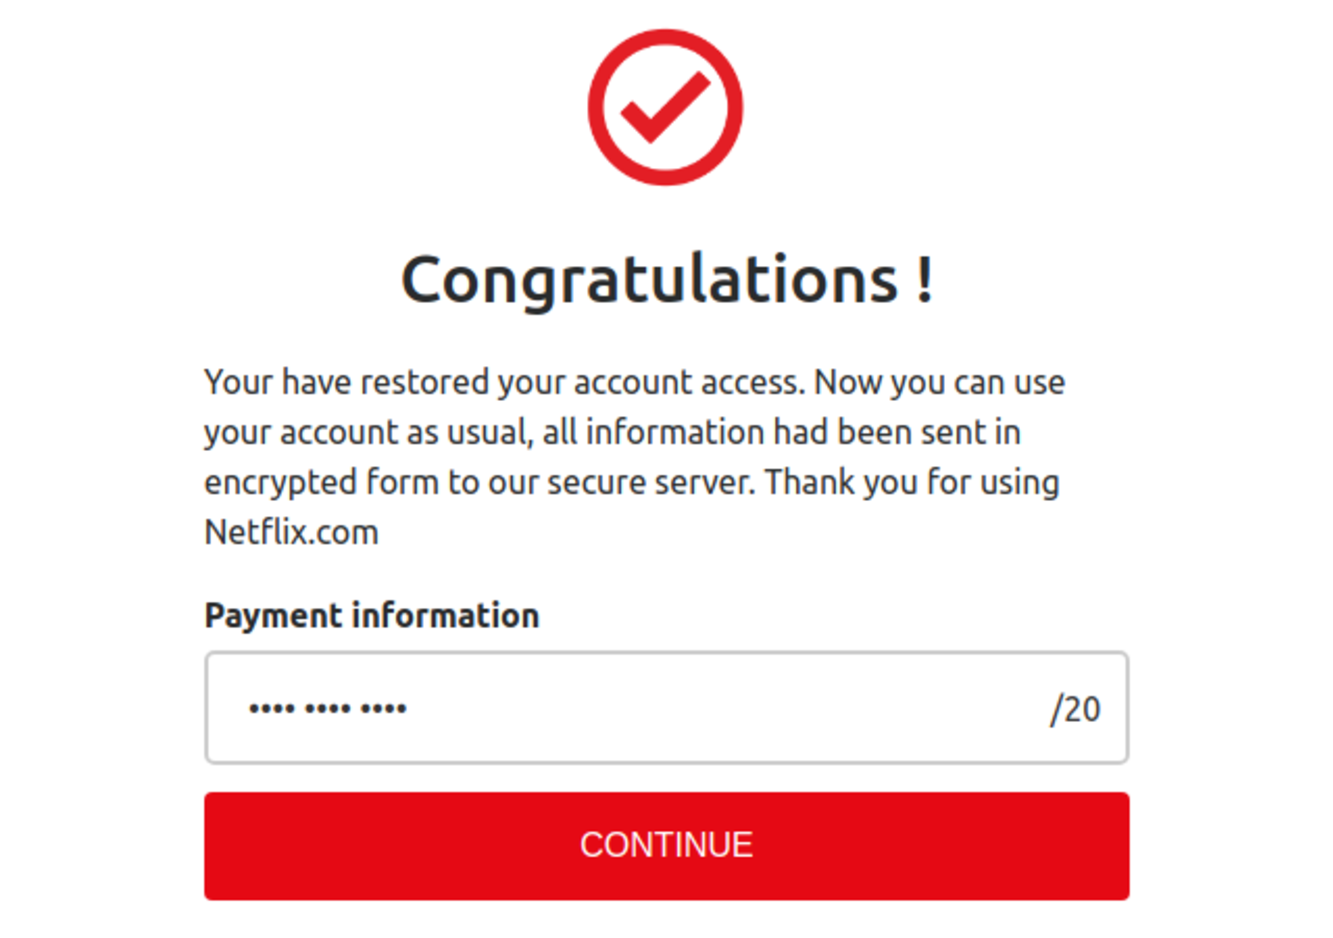
\includegraphics[width=\linewidth]{figs/netflix_n.pdf}
        \caption{Default browser visit.}
        \label{fig:normal}
	\end{subfigure}%
	\quad
	\begin{subfigure}[tb]{.31\textwidth}
		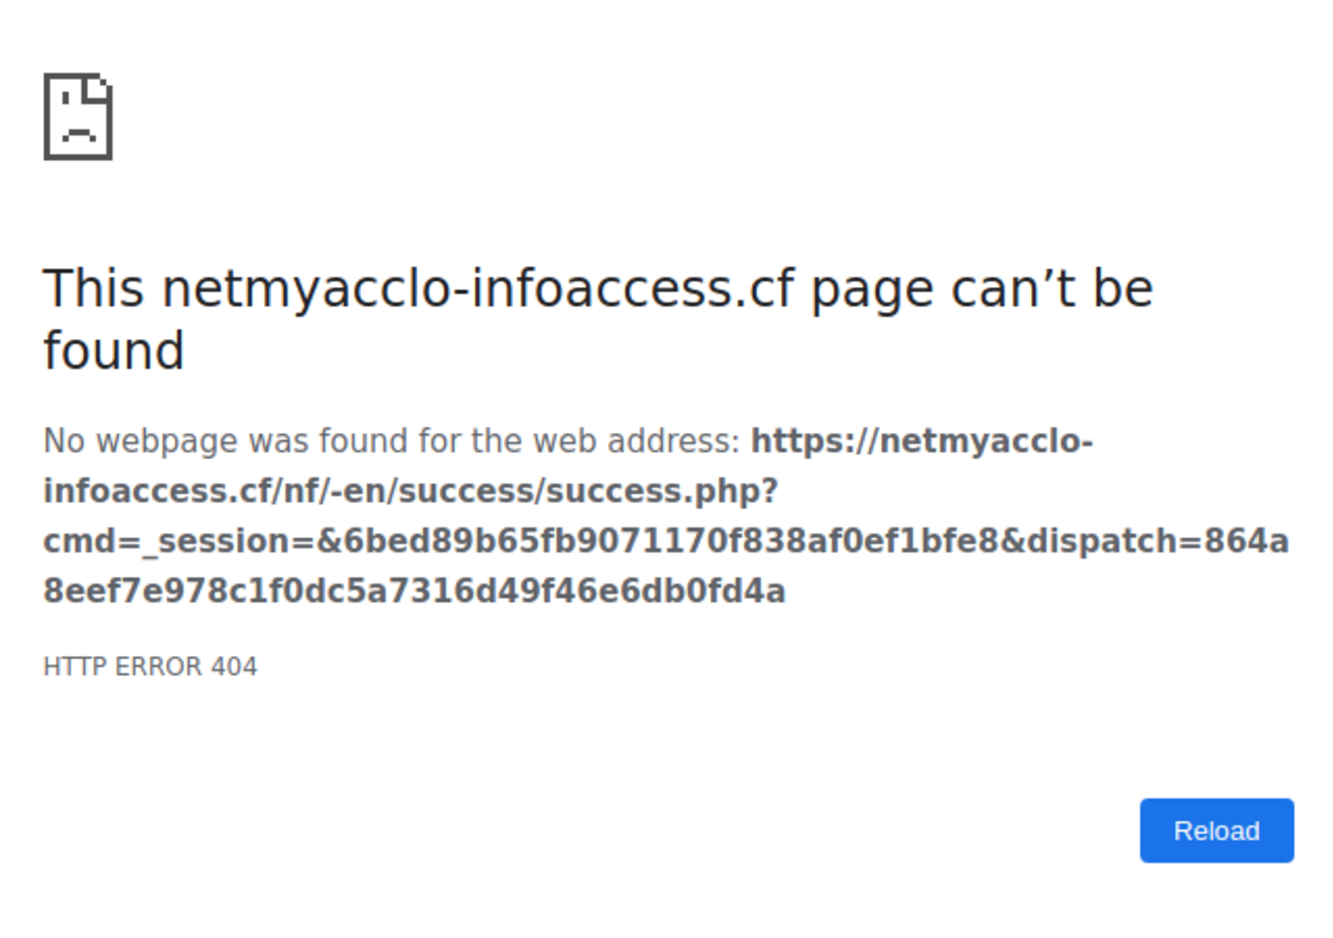
\includegraphics[width=\linewidth]{figs/netflix_sp.pdf}
        \caption{\spartacus browser visit with error.}
        \label{fig:sp1}
	\end{subfigure}%
	\quad
	\begin{subfigure}[tb]{.31\textwidth}
		
\includegraphics[width=\linewidth]{figs/netflix_sp2.png}
        \caption{\spartacus browser visit with content.}
        \label{fig:sp2}
	\end{subfigure}%
	\quad
% 	\vspace{-5pt}
	\caption{Web page contents from default and \spartacus'ed browser visits for a cloaked phishing website.}
	\label{fig:effectiveness}
% 	\vspace{-10pt}
\end{figure*}

We evaluate the effectiveness of \spartacus automatically by conducting an experiment where we visit same phishing websites with different configurations of browsers, one with default user setting, the other with \spartacus to mutate the profile.
We simulate the default setting browser as normal users and the one with \spartacus as users with our system.
The phishing URLs both browsers visit are from the APWG Dataset.
For each visit, we record the final landing web page content and URL.
Either a legitimate final URL or a non-malicious web page content indicates the success of \spartacus evading phishing content for users.
If there is still malicious content shown to \spartacus, it indicates that either the phishing website does not contain advanced evasion techniques, or \spartacus does not trigger them with current fingerprint.
For the first situation, the current anti-phishing ecosystem has proposed methodologies to mitigate basic phishing attacks with effectiveness and efficiency.
As for the second, we believe that by visiting the same website with different configurations of HTTP requests mutated by \spartacus, the evasion techniques embedded in the phishing website can be triggered eventually. 

We examined 160,728 phishing URLs from APWG from November 2020 to July 2021,
132,247 of which do not contain malicious content.
We consider an HTTP response benign if (1) its web page content does not contain maliciousness, such as phishy words or bad forms, according to CANTINA+~\cite{xiang2011cantina+};
(2) the response status code is an error one (4XX/5XX);
or (3) the destination domain is legitimate, excluding web hosting service domains.
\autoref{fig:effectiveness} demonstrates the difference of response web page content between default and \spartacus'ed browser visit for a cloaked phishing websites.
The content in~\autoref{fig:normal} shows the phishing content when a real person visits it.
On the other hand, when \spartacus appends a bot-looking string to the existing User-Agent, such as~\emph{googlebot}, the phishing server considers the visit as from an anti-phishing infrastructure.
Thus, it denies the request from \spartacus and an error web page is shown as~\autoref{fig:sp1}.
On the other hand, advanced phishing servers can redirect visit to a benign domain with status code of 200 instead of returning an error.
In this way, \spartacus'ed browser will receive web page contents such as~\autoref{fig:sp2},
which also indicates a successful evasion 
from \spartacus.

It shows that \spartacus can impersonate anti-phishing crawler and trigger the cloaking techniques of advanced phishing websites.
Because the web page content returned through \spartacus's visit does not contain any maliciousness, Internet users will not be trapped in the attack.

% \textcolor{blue}{eval result}

\subsection{Effectiveness of triggering words}

According to the design, the profile mutator of \spartacus selects one of 407 triggering words, following the order of their popularity in examined phishing kits.
So in this section, we evaluate the effectiveness of each triggering word on triggering fingerprinting cloaking techniques in phishing websites.

We test all the triggering words by appending each after the User-Agent string within \spartacus and then visiting the same phishing website.
Similarity to the evaluation of effectiveness of \spartacus, we also visit the website using a default browser as a comparison.
We conduct the experiment on 916 phishing websites.
Except ABC websites that show same content on all HTTP profiles,
DEF ones show web page differently between \spartacus'ed browser and default browser.

In DEF cloaked phishing websites, the triggering words have different evasion abilities.
Table X is the result of top 10 effective triggering words evading phishing content in \spartacus.
In the table, word XYZ has the most evasion record.
X\% of the cloaked phishing websites can be evaded by appending XYZ in the User-Agent using \spartacus.
Compared with the rank in~\autoref{tab:topsenswords}, it is X-th word in the list.
The high effectiveness of word XYZ confirms its high rank in the top used blocked words in the phishing kits.
Similarly, top effective words such as XXX, ZZZ, and YYY also have a high usage in phishing kits.
On the other hand, word XYZ and XXX combined can make all tested cloaked phishing websites return benign content to users.

The evaluation result shows that our triggering word list can evade phishing websites with fingerprinting cloaking techniques.
Furthermore, it indicates that a small number of triggering words can evade a myriad of cloaked phishing websites.


\subsection{Efficiency and Latency}

We need to make sure that \spartacus will not impact negatively on the user experience when they visit benign websites.
From the design of \spartacus, it will introduce latencies, including database query, HTTP profile mutation, and returned content inspection.
However, the latencies \spartacus introduces can be negligible.
Therefore, we conduct an experiment to measure the latency for the \spartacus system for the following three perspective, database query, profile mutation, and content inspection.
We leverage \emph{exthouse}~\cite{exthouse}, which analyzes the impact of a browser extension on web performance, as our test bench.
% We run exthouse with 1,000 phishing websites and 1,000 benign websites on two configurations of browsers, one with \spartacus, the other without, and compare the mean rendering time for each group of websites.
It contains five major measurements:
(1) Time to Interactive (TTI): the time it takes for the page to become fully interactive with the extension; 
(2) First Input Delay (FID $\Delta$): the time from when a user first interacts with the website to the time when the browser is actually able to begin processing event handlers in response to that interaction;
(3) Scripting Time (Scripting $\Delta$): the amount of time JavaScript execution in the extension;
(4) Long Task (Added Long Task): this value represents a sum of Long Tasks added by extension;
and (5) Extra CPU Consumption (Extra CPU Time): additional files in the extension need extra CPU consumption for each URL the browser visits.
The lower these three factors are, the better the website performs with the tested extension.
At last, \emph{exthouse} will score of the extension.
A higher score reflects a better performance of the extension.

\exthouse

\autoref{tab:exthouse} illustrates the metrics of top 10 Chrome extensions~\cite{exthouse} along with \spartacus when visiting benign and malicious websites under the inspection of \emph{exthouse}.
We test these extensions with 100 websites, including half benign and half malicious, and take the average into the metrics.
\spartacus has a score of 100, 20 ms FID, 0 scripting delta, and 800 ms of TTI when visiting benign websites.
The metrics of \spartacus visiting malicious websites also outscores those of other popular extensions.
Even though it takes long time to interact with the malicious website, it is still acceptable because \spartacus needs time to mutate the profile, which is still less than the time used consumed by other extensions.
Take \texttt{Avira Browser Safety} (ABS) as an example, it is an extension warning users if the website is unsafe.
However, it added long tasks and extra CPU time when visiting malicious websites.
As a similar type, \spartacus does not harden the CPU as ABS does.
At the same time, \spartacus can provide safe browsing for users.
The evaluation result means that with \spartacus, users can still interact with the website with minimum latency.
The inspection result shows that \spartacus out-scores popular Chrome extensions and does not impact the performance of websites, compared with other extensions.

\subsection{Impact on Benign Website}

Besides evading malicious content in phishing websites, \spartacus is also required to minimize the negative impacts on benign URL visit.
They can include ability of access the website, correct display of website layout, and correct functionalities of the website.
To evaluate the potential impacts to benign website, we conduct two experiments: Coarse-Grained and Fine-Grained.

\subsubsection{Coarse-Grained Experiment}

\coarsegrain

In Coarse-Grained experiment, we intend to evaluate if \spartacus system has negative impact on the access to the website or the website layout.
So we visit 60,848 (9.66\%) out of 629,843 URLs in Alexa Top One Million Domain List~\cite{AlexaTop1M} in both default and \spartacus'ed browsers.
We compare the web page screenshot and HTML similarity on the visited URLs.
The result is shown in~\autoref{tab:coarsegrain}.
After adopting~\Cref{alg:mutatelogic},
0.06\% (39) have different layouts and 
0.04\% (29) block the access from \spartacus'ed browser.

\begin{figure}[t]
    \centering
    \begin{subfigure}{0.48\linewidth}
        \centering
            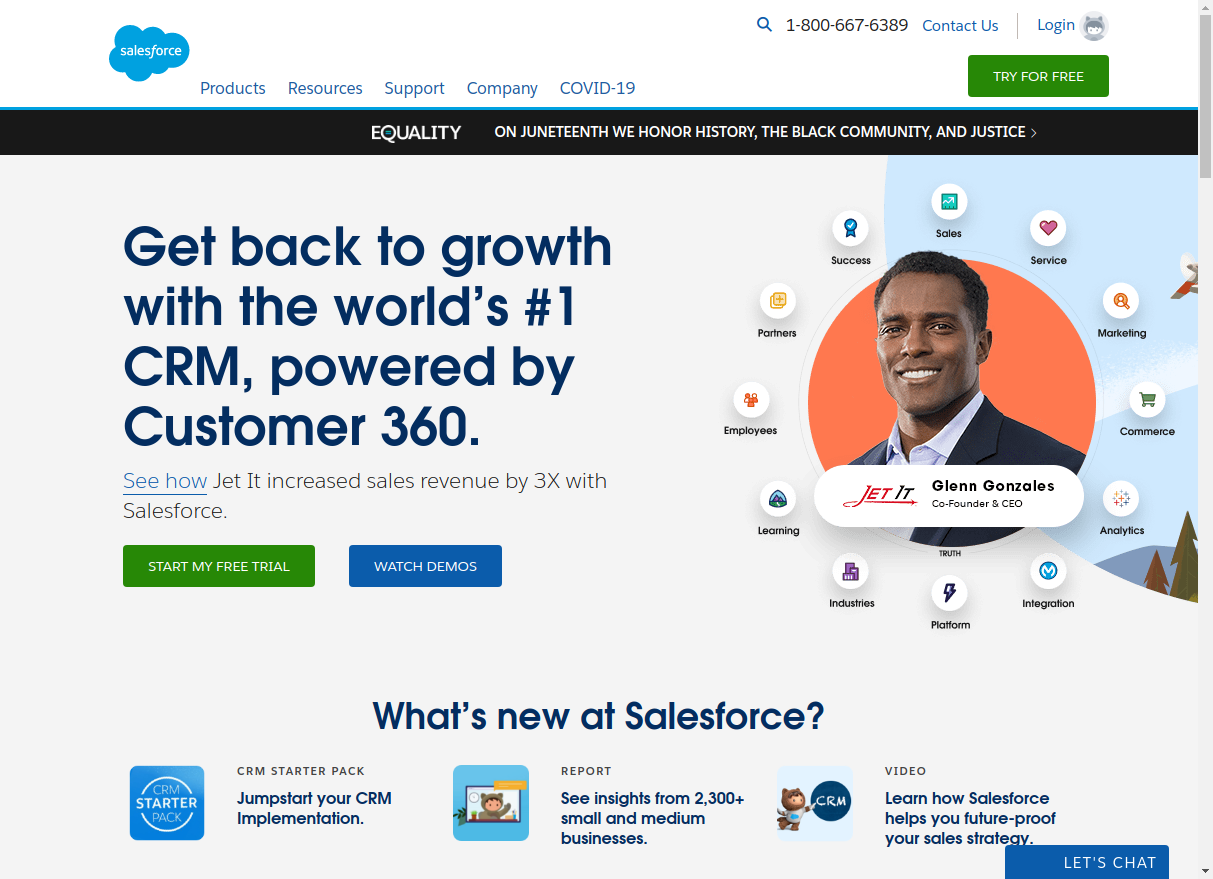
\includegraphics[width=\textwidth]{figs/38_normal.png}%
        \caption{Default browser visit.}
        \label{fig:coarse_normal}
    \end{subfigure}
    ~
    \begin{subfigure}{0.48\linewidth}
        \centering
            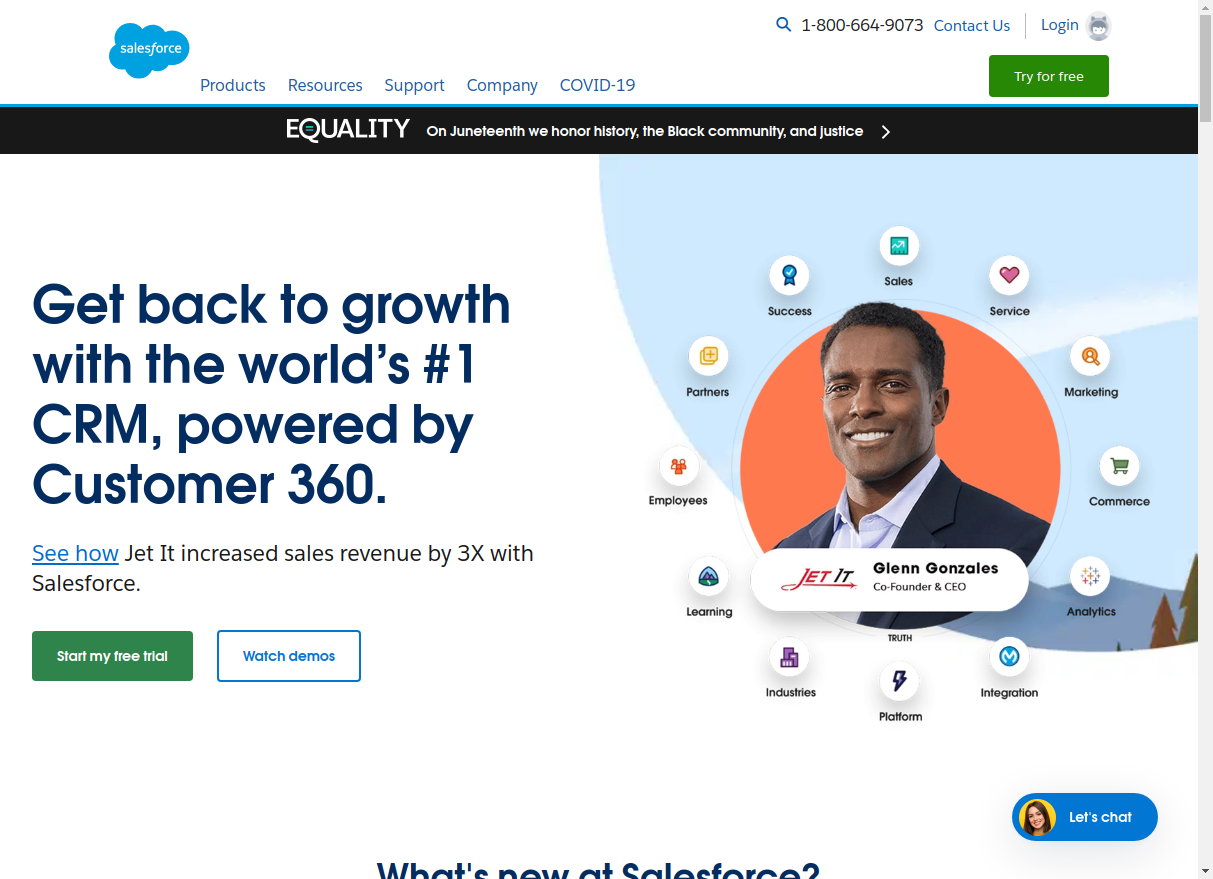
\includegraphics[width=\textwidth]{figs/38_sp.png}
        \caption{\spartacus visit}
        \label{fig:coarse_sp}
    \end{subfigure}
    
    \caption{Difference due to the shape of buttons.}
    \label{fig:coarse}
    % \vspace{-10pt}
\end{figure}

\begin{figure}[t]
    \centering
    \begin{subfigure}{0.48\linewidth}
        \centering
            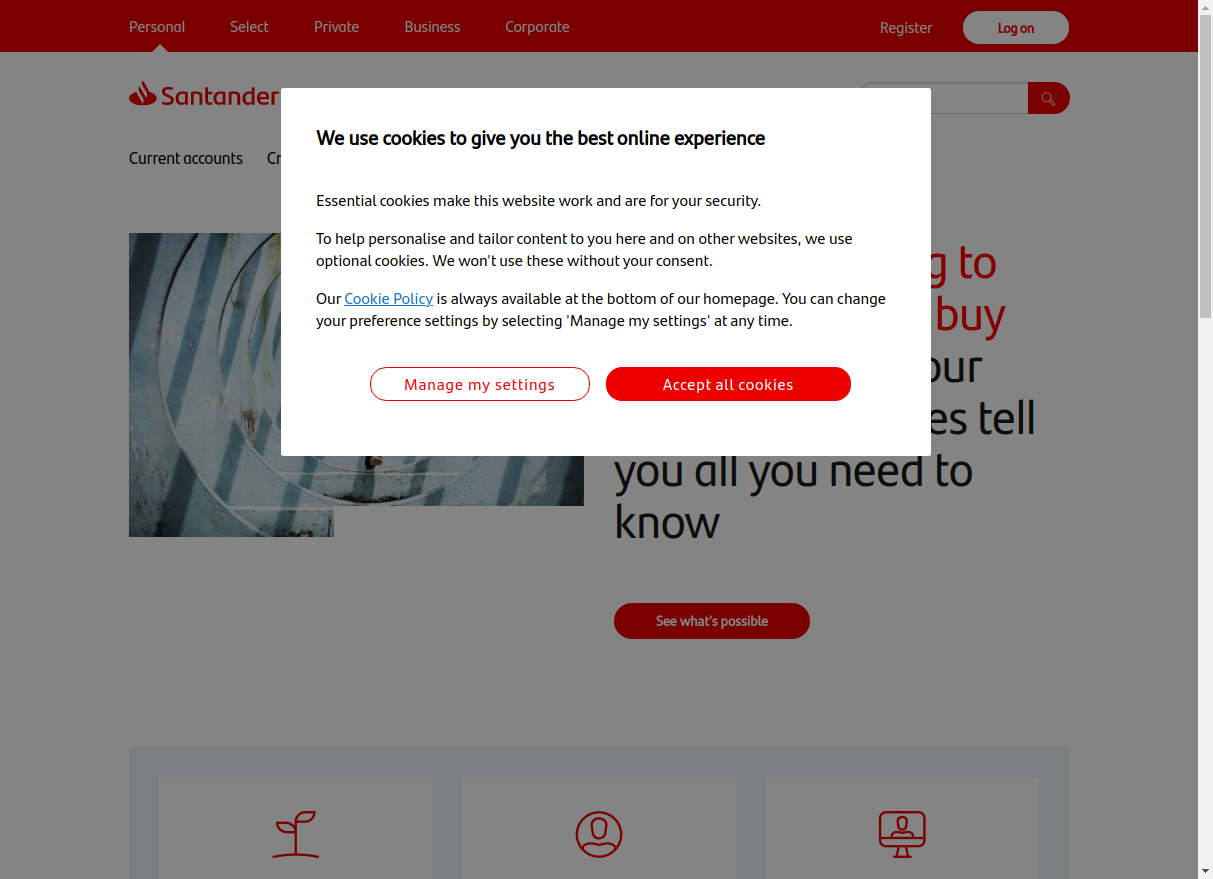
\includegraphics[width=\textwidth]{figs/2306_normal.png}%
        \caption{Default browser visit.}
        \label{fig:2306_normal}
    \end{subfigure}
    ~
    \begin{subfigure}{0.48\linewidth}
        \centering
            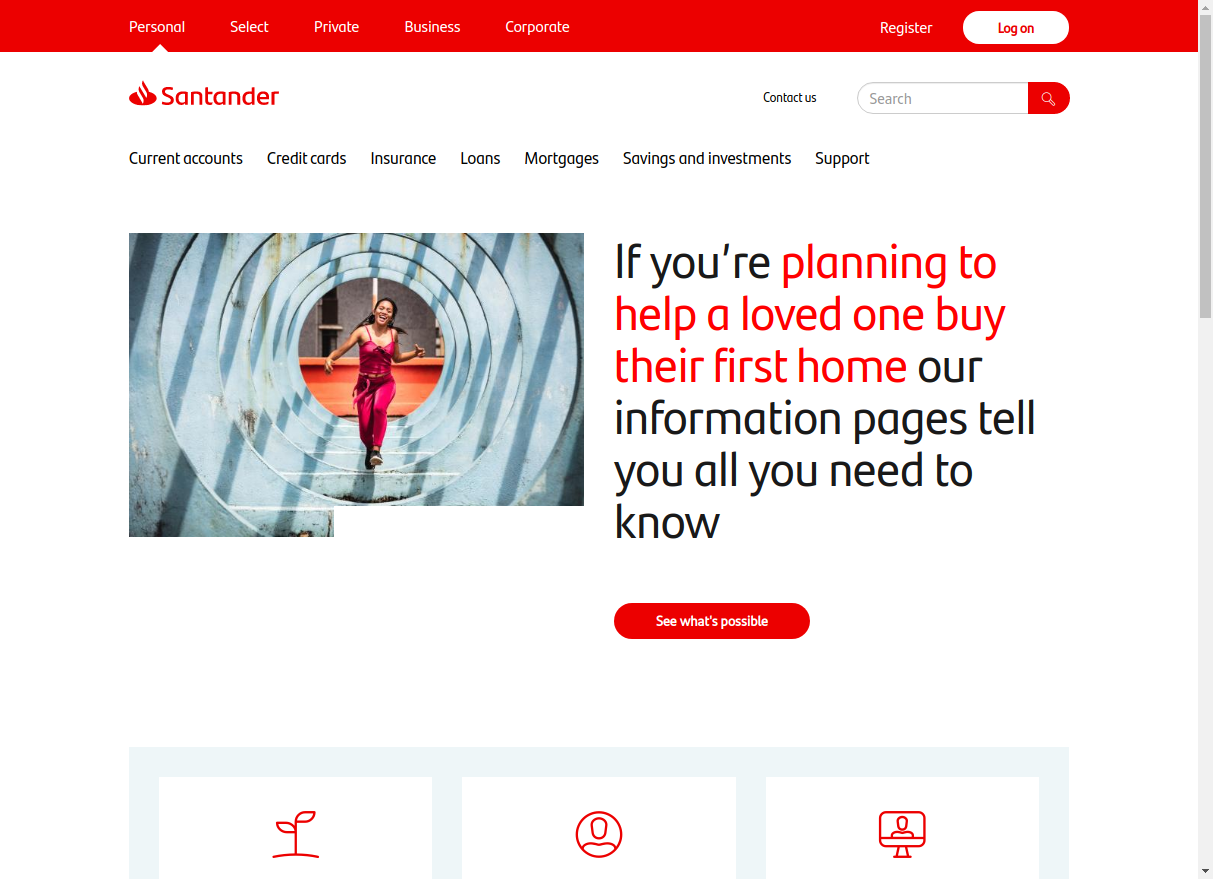
\includegraphics[width=\textwidth]{figs/2306_sp.png}
        \caption{\spartacus visit}
        \label{fig:2306_sp}
    \end{subfigure}
    
    \caption{Difference due to popup.}
    \label{fig:2306}
    % \vspace{-10pt}
\end{figure}

We first examine the reason why \spartacus'ed browser show different layouts from the default browser.
And we find that although the screenshot and HTML similarity is not high between default and \spartacus browser visits,
to people, such difference does not impact them using or browsing the website.
For example, two web pages are different in terms of screenshot similarity between default and \spartacus browser visits shown in~\autoref{fig:coarse}.
The difference is due to the shape of buttons and different of background color.
% The change is on the scrolling promotion ads in the \texttt{div} tag.
% When the screenshot was captured in default visit, Ad One happened to show;
% and another Ad was in the way when \spartacus took the screenshot.
Similarly, in~\autoref{fig:2306}, a window popped up to ask for the permission of cookie in default browser, but did not in \spartacus's visit.
The cookie request pop-up is missing in \spartacus browser, not due to the extension itself, but because we visit the same website 10 times in different browsers without \spartacus, only for 3 times the pop-up appeared.
Even though our evaluation script can distinguish the difference between visits from two browsers,
users will not perceive that.
They can normally interact with the websites with \spartacus providing phishing-evading services.
% , which indicates that \spartacus does not make users perceive the difference, even if it has 




With applying~\Cref{alg:mutatelogic}, we evaluated \spartacus based on the threshold and find that 29 legitimate domains show different web page content on default and \spartacus'ed browsers, as listed in~\autoref{tab:coarsegrain}.
Hence, only 0.04\% of 60,848 domains are falsely evaded.
It is because the 29 domains do not fall into the high reputation group of \spartacus's non-mutation criteria.
As one possible mitigation, we provide a channel for users to report falsely evaded websites.
Once receiving the report from the client side, we will conduct manual inspection and whitelist the false-positives.
% Additionally, 39 of the domains show different layouts between default and \spartacus browsers.
% As we discussed above, such difference will not affect the activities of normal users,
% but after applying~\Cref{alg:mutatelogic}, \spartacus and normal browsers perform more alike on benign domains.
As comparison, phishing URLs can still be evaded through \spartacus because they all triggered the condition to invoke \emph{mutate\_http\_profile()}.

\subsubsection{Fine-Grained Experiment}

\finegrain


In Fine-Grained experiment, we aim to exercise and evaluate the operation of websites visited through \spartacus.
It was inspired by the methodology used by Snyder et al.~\cite{snyder2017most} and Trickel et al.~\cite{trickel2019everyone}.
This methodology concentrates on the operation of a website from the perspective of the user.
Even though \spartacus may introduce an error to a website while users do not perceive any difference when browsing, then we consider that \spartacus does not impact negatively on the website.
% evaluate potential impact \spartacus brings on the functionalities of benign domains.
This method of evaluation focuses more on potential impact \spartacus brings on the functionalities of benign domains than how \spartacus works.
And it was performed by the authors manually.

The experiment includes the evaluation of visibility of websites and interactions between visitor and the website.
It brings an additional metric that evaluates how \spartacus will influence users' daily activities.
There are four steps in the experiment.
(1) We open legitimate domains in a browser with \spartacus installed and also in one with default settings.
(2) We inspect the accessibility of the website, similar to the Coarse-Grained experiment.
(3) After the success of web page content retrieval, we compare the layouts between different visit.
(4) We interact with links, buttons, and other activities such as register/login, online chat, or shopping to make sure that their functionalities perform correctly.
(5) At last, we test the authentication functionality to make sure that \spartacus extension will not impact it.

We randomly selected 60 domains from Alexa Top One Million List, especially 20 every 200 thousands.
The result is displayed in~\autoref{tab:finegrain}.
As a comparison, default browser has the same result as that of \spartacus.
Among the 60 legitimate domains, we can access 58 of them.
Two domains are inaccessible even in the default browser, so we suspect them offline already.
For the accessible 58 domains,
we follow the steps mentioned above to inspect them.
All of them have the same layout as the visit from the default browser.
Then we interact the 58 websites by clicking the buttons, chatting online, and adding items into the cart if it is a shopping website.
All 58 websites performed well.
At last, we register an account on 15 websites and they all allow us to do so.
Even though we can successfully register an account, we still need to make sure that we can log in properly with those accounts to test the authentication process under \spartacus.
The result shows that all the accounts we registered during the Fine-Grained experiment can be logged in successfully.
It means that the \spartacus system does not impact the authentication process in the website.

In summary, with the results retrieved from both coarse- and fine-grained experiment, we can summarize that \spartacus does not impact the accessibility and visibility on high reputation or long age domains, or its top reviewed subdomains.
Besides, for domains who can be accessed and displayed properly, the functionalities including links, buttons, and registration and authentication in the websites will not be affected.
Therefore, \spartacus can protect users from visiting advanced phishing websites while keep their normal browsing activities.

% \noindent
% \textbf{Database Query}.
% According to the e

% \noindent
% \textbf{Profile Mutation}.

% \noindent
% \textbf{Content Inspection}.

% \subsection{Privacy}


\section{Related Work}

Researchers have studied phishing for several decades.
They have proposed several methodologies to detect phishing attacks based on one or some of features from URL, content, and etc, and then warn users before visiting the deceptive websites.
Some work analyzes URL of a suspicious website based on the lexical features or URL ranking to determine the maliciousness of the site~\cite{blum2010lexical, le2011phishdef, khonji2012enhancing, feroz2015phishing}.
Others collect web page content and detect phishing websites with textual and visual similarity features~\cite{zhang2007cantina, zhang2011textual, dunlop2010goldphish}.
Combining with available features including both URL and web page content, researchers have developed blacklist based anti-phishing systems such as Google Safe Browsing~\cite{whittaker2010large} to protect Internet users from visiting suspicious websites.
All the proposed methodologies in the past, however, have a limitation that they are detection systems, and require certain features to classify the maliciousness,
which takes long time to output and hence leaves phishers golden hour to harvest.

With the large-scale implementation of cloaking techniques in phishing attacks~\cite{oest2020sunrise, oest2020phishtime, oest2019phishfarm, oest2018inside}, researchers realize that the sophisticated phishing attacks are responsible for substantial portion of damage and that the whole ecosystem should prioritize on mitigating phishing with evasion techniques.
The cloaking techniques make the path of anti-phishing tougher for the proposed methodologies because it becomes more and more difficult to retrieve phishing content, which most anti-phishing systems depend on.
With very limited amount of features of a suspicious website, the system cannot determine precisely the maliciousness.

Therefore, analysis and detection of server-side
% ~\cite{wang2011cloak, invernizzi2016cloak} 
and client-side
% 
cloaking techniques have been proposed to fight against such sophistications.
For client-side cloaking techniques, Zhang et al.~\cite{zhang2021crawlphish} proposed CrawlPhish to force-execute JavaScript snippets in the payload to reveal malicious content.
As for server-side cloaking in phishing, previous work~\cite{wang2011cloak, invernizzi2016cloak, oest2018inside} can only categorize types of server-side cloaking through analysis of compromised phishing kits.
The whole security community does not have an efficient and effective methodology to mitigate them.
Phishers can always evolve to add new crawler-looking features in the phishing kits to block any suspicious visit.


% All the proposed methodologies, however, have a limitation that they only provide a pain-relief pills to certain symptoms of phishing attacks, such as suspicious URL, similar layout as the impersonated website, and cloaking techniques.

% Furthermore, as phishers have been developing advanced cloaking techniques, it becomes more and more difficult to retrieve phishing content, which most anti-phishing systems depend on.

% Therefore, with the contribution of previous studies on phishing symptoms, 
Considering the nature and prevalence of cloaked phishing websites~\cite{oest2018inside, oest2019phishfarm},
our work provides a vaccine to neutralizing advanced phishing-virus.
Rather than trying best to bypass cloaking techniques in phishing websites, \spartacus deliberately triggers them and hence retrieve benign content to show to users.
Our framework is also extendable and always up-to-date by adding fingerprints that researchers will find in the future.



% %-------------------------------------------------------------------------------
% \section{Introduction}
% %-------------------------------------------------------------------------------

% A paragraph of text goes here. Lots of text. Plenty of interesting
% text. Text text text text text text text text text text text text text
% text text text text text text text text text text text text text text
% text text text text text text text text text text text text text text
% text text text text text text text.
% More fascinating text. Features galore, plethora of promises.

% %-------------------------------------------------------------------------------
% \section{Footnotes, Verbatim, and Citations}
% %-------------------------------------------------------------------------------

% Footnotes should be places after punctuation characters, without any
% spaces between said characters and footnotes, like so.%
% \footnote{Remember that USENIX format stopped using endnotes and is
%   now using regular footnotes.} And some embedded literal code may
% look as follows.

% \begin{verbatim}
% int main(int argc, char *argv[]) 
% {
%     return 0;
% }
% \end{verbatim}

% Now we're going to cite somebody. Watch for the cite tag. Here it
% comes. Arpachi-Dusseau and Arpachi-Dusseau co-authored an excellent OS
% book, which is also really funny~\cite{arpachiDusseau18:osbook}, and
% Waldspurger got into the SIGOPS hall-of-fame due to his seminal paper
% about resource management in the ESX hypervisor~\cite{waldspurger02}.

% The tilde character (\~{}) in the tex source means a non-breaking
% space. This way, your reference will always be attached to the word
% that preceded it, instead of going to the next line.

% And the 'cite' package sorts your citations by their numerical order
% of the corresponding references at the end of the paper, ridding you
% from the need to notice that, e.g, ``Waldspurger'' appears after
% ``Arpachi-Dusseau'' when sorting references
% alphabetically~\cite{waldspurger02,arpachiDusseau18:osbook}. 

% It'd be nice and thoughtful of you to include a suitable link in each
% and every bibtex entry that you use in your submission, to allow
% reviewers (and other readers) to easily get to the cited work, as is
% done in all entries found in the References section of this document.

% Now we're going take a look at Section~\ref{sec:figs}, but not before
% observing that refs to sections and citations and such are colored and
% clickable in the PDF because of the packages we've included.

% %-------------------------------------------------------------------------------
% \section{Floating Figures and Lists}
% \label{sec:figs}
% %-------------------------------------------------------------------------------


% %---------------------------
% \begin{figure}
% \begin{center}
% \begin{tikzpicture}
%   \draw[thin,gray!40] (-2,-2) grid (2,2);
%   \draw[<->] (-2,0)--(2,0) node[right]{$x$};
%   \draw[<->] (0,-2)--(0,2) node[above]{$y$};
%   \draw[line width=2pt,blue,-stealth](0,0)--(1,1)
%         node[anchor=south west]{$\boldsymbol{u}$};
%   \draw[line width=2pt,red,-stealth](0,0)--(-1,-1)
%         node[anchor=north east]{$\boldsymbol{-u}$};
% \end{tikzpicture}
% \end{center}
% \caption{\label{fig:vectors} Text size inside figure should be as big as
%   caption's text. Text size inside figure should be as big as
%   caption's text. Text size inside figure should be as big as
%   caption's text. Text size inside figure should be as big as
%   caption's text. Text size inside figure should be as big as
%   caption's text. }
% \end{figure}
% %% %---------------------------


% Here's a typical reference to a floating figure:
% Figure~\ref{fig:vectors}. Floats should usually be placed where latex
% wants then. Figure\ref{fig:vectors} is centered, and has a caption
% that instructs you to make sure that the size of the text within the
% figures that you use is as big as (or bigger than) the size of the
% text in the caption of the figures. Please do. Really.

% In our case, we've explicitly drawn the figure inlined in latex, to
% allow this tex file to cleanly compile. But usually, your figures will
% reside in some file.pdf, and you'd include them in your document
% with, say, \textbackslash{}includegraphics.

% Lists are sometimes quite handy. If you want to itemize things, feel
% free:

% \begin{description}
  
% \item[fread] a function that reads from a \texttt{stream} into the
%   array \texttt{ptr} at most \texttt{nobj} objects of size
%   \texttt{size}, returning returns the number of objects read.

% \item[Fred] a person's name, e.g., there once was a dude named Fred
%   who separated usenix.sty from this file to allow for easy
%   inclusion.
% \end{description}

% \noindent
% The noindent at the start of this paragraph in its tex version makes
% it clear that it's a continuation of the preceding paragraph, as
% opposed to a new paragraph in its own right.


% \subsection{LaTeX-ing Your TeX File}
% %-----------------------------------

% People often use \texttt{pdflatex} these days for creating pdf-s from
% tex files via the shell. And \texttt{bibtex}, of course. Works for us.

% %-------------------------------------------------------------------------------
% \section*{Acknowledgments}
% %-------------------------------------------------------------------------------

% The USENIX latex style is old and very tired, which is why
% there's no \textbackslash{}acks command for you to use when
% acknowledging. Sorry.

% %-------------------------------------------------------------------------------
% \section*{Availability}
% %-------------------------------------------------------------------------------

% USENIX program committees give extra points to submissions that are
% backed by artifacts that are publicly available. If you made your code
% or data available, it's worth mentioning this fact in a dedicated
% section.

% %-------------------------------------------------------------------------------
\bibliographystyle{plain}
\bibliography{reference.bib}
% \bibliography{\jobname}

%%%%%%%%%%%%%%%%%%%%%%%%%%%%%%%%%%%%%%%%%%%%%%%%%%%%%%%%%%%%%%%%%%%%%%%%%%%%%%%%
\end{document}
%%%%%%%%%%%%%%%%%%%%%%%%%%%%%%%%%%%%%%%%%%%%%%%%%%%%%%%%%%%%%%%%%%%%%%%%%%%%%%%%

%%  LocalWords:  endnotes includegraphics fread ptr nobj noindent
%%  LocalWords:  pdflatex acks
